\chapter{Анализ современных трактов приема сверхширокополосных сигналов}

\section{Главный тракт приема сверхширокополосных сигналов}
\subsection{Супергетеродинный приемник}

\subsection{Приемник прямого преобразования}

\section{Факторы ухудшающие быстродействие обработки сверхширокополосных сигналов}

\section{Источники возникновения ошибок и расхождений фазы сигналов, подходы к уменьшению их влияния}

\section{Анализ современных методов построения сверхширокополосных малошумящих усилителей}

Основными параметрами МШУ являются:
\begin{itemize}
	\item Коэффициент шума;
	\item Коэффициент усиления;
	\item Точка одноцебельной компрессии;
	\item Точка интермодуляции (перехвата) третьего порядка;
	\item Потребляемая мощность.
\end{itemize}

Согласно формуле Фрииса \eqref{eq:friise} основной вклад в шумовую характеристику приемного тракта вносит первый усилительный каскад.

\begin{equation}
F_{total} = F_1 + \frac{{F_2 - 1}}{G_1} + \frac{{F_3 - 1}}{G_1 G_2} + \frac{F_4 - 1}{G_1 G_2 G_3} + ... + \frac{F_N - 1}{\prod\limits_{N=1} G_N},
\label{eq:friise}
\end{equation}
где \(F_{total}\) -- суммарный коэффициент шума приемного тракта, \(F_N\) -- коэффициент шума \textit{N}-го каскада, \(G_N\) -- коэффициент усиления \textit{N}-го каскада.

Из выражения \eqref{eq:friise} следует, что для удовлетворения требований к МШУ, перечисленных выше, необходимо снижать коэффициент шума каждого каскада при одновременном увеличении коэффициента усиления. Исходя из данного наблюдения возникает противоречие, т.к. для повышения коэффициента усиления необходимо увеличивать ток потребления усилителя. При увеличении коэффициента усиления, ухудшается линейность усилителя, следовательно, уменьшается динамический диапазон устройства. При попытке улучшить линейность усилителя, уменьшается коэффициент усиления каждого каскада, в следствии чего возрастает коэффициент шума.

Из-за подобной связности какого-либо параметра с любым другим практически не существует универсальных способов и схем, позволяющих разработать усилитель удовлетворяющий всем требуемым характеристикам технического задания.

\subsection{Источники возникновения шумов в полупроводниковых устройствах}
В данном разделе рассмотрим источники возникновения шума в полевых и биполярных транзисторах, а также методы снижения их вклада в общую шумовую картину.

\subsubsection{Температурный шум (Thermal Noise)}

\subsubsection{Дробовый шум (Shot Noise)}

\subsubsection{\(1/f\) Фликер шум (Flicker Noise)}

\subsection{Принцип действия широкополосного малошумящего усилителя}

\subsection{Входное согласование по мощности}
Качество входного согласования выражается в значении отраженной мощности или возвратных потерь, которые для входного сопротивления МШУ \(Z_{in}\) и сопротивления источника \(R_S\) определяются как \eqref{eq:gamma}

\begin{equation}
\label{eq:gamma}
\Gamma = {\Bigg| \frac{Z_{in} - R_S}{Z_{in} + R_S} \Bigg|}^2
\end{equation}

С целью оптимизации входной цепи МШУ по наименьшему вкладу в общий коэффициент шума, \(\Gamma\) может не согласововаться с выходным сопротивлением источника. Таким образом, выбор рабочей точки \(\Gamma_{opt}\) должен обеспечивать компромисс между вкладом в общую шумовую характеристику и согласованием по мощности.

\subsection{Первый каскад МШУ}
Так как основное влияние на шумовые характеристики оказывает первый каскад усиления, необходимо максимально снизить количество вносимых шумов цепями согласования, входным транзистором и т.п.

В качестве усилительного каскада могут применяться схемы включения транзистора:
\begin{itemize}
	\item Общий эмиттер (общий исток);
	\item Общая база (общий затвор);
	\item Каскодная схема -- общий эмиттер-общая база (общий исток-общий затвор).
\end{itemize}

При работе на частотах диапазона Ka (27 -- 40 ГГц) и выше, каскодная схема и общая база используются реже из-за ухудшающихся шумовых характеристик и, в случае каскода, повышенной промежуточной емкостью в узле соединения двух транзисторов, что приводит к значительному ухудшению усилительных свойств каскада.

\subsection{МШУ с дифференциальным выходом}

\subsection{Возникновение и методы снижения влияния нелинейных эффектов}

\section{Усилитель-ограничитель}

\section{Усилитель с регулировкой коэффициента усиления}

\section{Широкополосный активный фазовращатель}

\section{Сверхширокополосные смесители}

\subsection{Сверхширокополосные смесители в интегральном исполнении}

\subsection{Шумы в полупроводниковых смесителях}

\section{Фильтры промежуточной частоты}

\chapter{Схемотехнический расчет СФ-блоков}

\section{Устройство выборки-хранения}
Определим мощность шумов квантования идеального АЦП с разрядностью \(N\) и размахом полной шкалы \(V_{FS}\)
\[ {P_{q}}^2 = \frac{\Delta^2}{12}\]
если \(\Delta = \dfrac{V_{FS}}{2^N}\), тогда \( {P_q}^2 = 223.52~\mathrm{pW} \).

\section*{Технические требования к аналого-цифровому преобразователю}
Характеристики приведены в Табл.\ref{tab:Parameters}.
\begin{table}[h]
	\caption[Характеристики разрабатываемого АЦП]{Характеристики разрабатываемого АЦП}
	\label{tab:Parameters}
	\centering
	\begin{tabular}{rrr}
		\toprule
		\textbf{Параметр}      & \textbf{Значение} & \textbf{Единица измерения}\\
		\midrule
		\(N\)                 &   14      & Бит\\
		\(F_{clk}\)           &   250     & МГц\\
		\(V_{FS}\)            &   1.2     & В\\
		\(V_{CM_{in}}\)                   &   600     & мВ\\
		\(FPBW\) (Full Power Bandwidth)   & 750 & МГц\\
		\bottomrule
	\end{tabular}
\end{table}

УВХ построено на базе МОП ключа Q1 с цепью смещения напряжения затвора \(V_{gs1}\), позволяющей снизить нелинейность ключа, возникающую из-за неполного <<закрытия>> или <<открытия>> канала.

\begin{figure}[ht]
	\centering
	\begin{circuitikz}[american, scale=1, transform shape]
	\ctikzset{tripoles/mos style/arrows}
	\ctikzset{bipoles/thickness=2}
	\ctikzset{tripoles/pmos style/emptycircle}
	\def\killdepth#1{{\raisebox{0pt}[\height][0pt]{#1}}} \path (0,0) -- (2,0); % bounding box
	\draw (0,0) node[nmos,rotate=-90](Q1){\rotatebox{90}{Q1}};
	\draw (Q1.D) to [short, l=Out, -] ++(2,0) to[C, l2^=$C_h$ and 4 pF]
	++(0,-1) node[ground](GND){};    ++(0,-1) node[ground](GND){};
	
	
	\draw ++(-3,0) coordinate(in) node[left](vi1){$v_i=v_1$} [short, l=Input, o-] to (Q1.S);
	\draw (in) ++(2,0) [short, *-] to ++(0,2) node[nmos, rotate=-90, anchor=D](Q2){\rotatebox{90}{Q2}};
	\draw (Q2.G) [short, -] to (Q2.G -| Q1.G) [short,-] to (Q1.G);
	\draw (Q2.S) node[nmos, rotate=-90, anchor=D](Q3){\rotatebox{90}{Q3}};
	\draw (Q3.D) [short, *-] to [C] ++(0, 4) coordinate(temp);
	\draw (temp) node[pmos, bulk, rotate=90, anchor=D, xscale=-1](Q4){\scalebox{1}[-1]{\rotatebox{90}{Q4}}};
	\draw (Q4.S) [short, -, l_=VDD] to ++(-1,0) coordinate(VDD);
	\draw (Q4.bulk) [short, -*] to (Q4.D);
	\draw (Q4.D) node[pmos, bulk, rotate=90, anchor=S, xscale=1](Q5){\rotatebox{-90}{Q5}};
	\draw (Q5.bulk) [short, -] to (Q5.S);
	\draw (Q5.D) [short, -] to (Q5.D -| Q1.G) to (Q2.G -| Q1.G);
	\node [circ] at (Q2.G -| Q1.G){};
	\draw (Q5.D -| Q1.G) node[nmos, anchor=S, rotate=-90, xscale=-1](Q6){\scalebox{1}[-1]{\rotatebox{-90}{Q6}}};
	\node [circ] at (Q5.D -| Q1.G){};
	\draw (Q6.D) [short, l=GND, -] to ++(1,0) coordinate(GND);
	\draw (Q4.G) [short, -] to (Q4.G -| Q6.S) to (Q6.S);
	
	\draw (Q3.G) [short, -, l_=clk] to (Q3.G -| VDD);
	\draw (Q3.S) [short, -, l=GND] to ++(-1,0);
	
	\draw (Q5.G) [short, -] to (Q6.G);
	\node [circ] at (Q6.G){};
	\draw (Q6.G) [short,-,l=clk] to (Q6.G -| GND);
	
	%COOOOOORDS
	%\path (temp) \coord(temp);
\end{circuitikz}
	
	\caption{Схема устройства выборки-хранения}
	\label{ct:bootstrapped_switch}
\end{figure}

\begin{figure}[ht]
	\centering
	\begin{circuitikz}[american, scale=1, transform shape]
	\def\killdepth#1{{\raisebox{0pt}[\height][0pt]{#1}}} \path (0,0) -- (2,0); % bounding box
	\ctikzset{transistors/arrow pos=end}
	\ctikzset{transistors/scale=1}
	\ctikzset{resistors/scale=0.8}
	\ctikzset{capacitors/scale=0.8}
	
	\draw (0, 0) node[npn, anchor=B](Q1){Q1};
	\draw (Q1.B) [short, *-] to [C] ++(-2,0) [short, -o, l=RF Input] to ++(-1,0);
	\draw (Q1.B) [short, -] to ++(0, 1) to [R=\(R_{feedback}\)] ++(0, 2) to [C=\(C_{feedback}\)] ++(0, 2) coordinate(tmp) [short, -*] to (Q1.C |- tmp);
	\draw (Q1.C |- tmp) to[R, l_=\(R1\)] ++(0, 3) node[vcc](VCC){\(V_{CC}=2.5 V\)};
	\draw (Q1.C |- tmp) [short, -] to (Q1.C);
	\draw (Q1.E) [short, -] to [R, l=\(R_{E}\)] +(0,-2) node[ground](GND){};
	
	\draw (Q1.C) ++(0,1) [short, *-] to [C] ++(2,0) coordinate(tmp);
	\draw (tmp) node[npn, anchor=B](Q2){Q2};
	\draw (Q2.E) to[R] ++(0,-2) node[ground](GND){};
	\draw (Q2.E) [short, *-] to ++(1,0) coordinate(tmp);
	\draw (tmp) to [C] ++(0,-2) node[ground](GND){};
	\draw (Q2.C) node[npn, anchor=E](Q3){Q3};
	\draw (Q3.C) to[R] ++(0,2) node[vcc](VCC){\(V_{CC}\)};
	\draw (Q3.B) [short, -] to (Q3.B |- VCC) [short, -*] to (VCC);
	
	\draw (Q3.C) [short, *-] to [C] ++(2,0) coordinate(tmp);
	\draw (tmp) node[npn, anchor=B](Q4){Q4};
	\draw (Q4.C) to [R] ++(0,2) node[vcc](VCC){\(V_{CC}\)};
	\draw (Q4.E) [short, -] to ++(0, -1) to ++(2,0) coordinate(tmp) to [R] ++(0,-2) node[ground](GND){};
	\draw (tmp) [short, *-] to ++(2, 0) coordinate(tmp);
	\draw (tmp) [short, -] to ++(0, 1) coordinate(tmp);
	\draw (tmp) node[npn, anchor=E, xscale=-1](Q5){\scalebox{-1}[1]{Q5}};
	\draw (Q5.C) to [R] ++(0,2) node[vcc](VCC){\(V_{CC}\)};
	\draw (Q5.B) [short, -] to [C] ++(0,-2) node[ground](GND){};
	
	\draw (Q4.C) [short, *-o, l=\(v_{out-}\)] to ++(1.2,0);
	\draw (Q5.C) [short, *-o, l_=\(v_{out+}\)] to ++(-1.2,0);
	
	%COOOOOORDS
	%\path (tmp) \coord(tmp);
\end{circuitikz}
	
	\caption{Схема электрическая принципиальная рассматриваемого МШУ}
	\label{ct:lna_balun_wo_bias}
\end{figure}

\begin{figure}[ht]
	\centering
	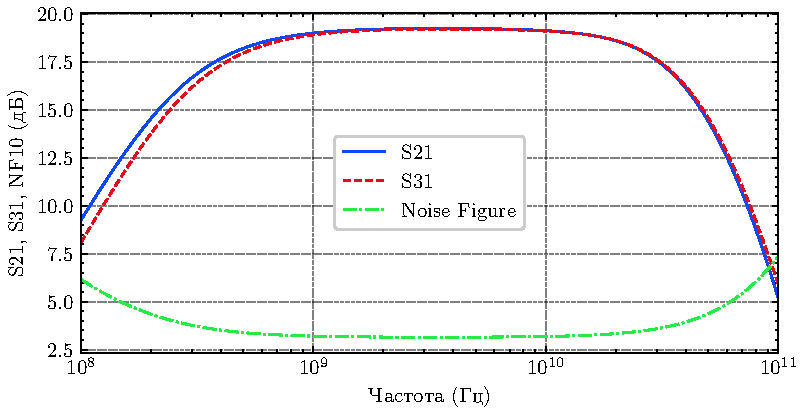
\includegraphics[width=0.8\linewidth]{lna_gain_nf.pdf}
	
	\caption{Результаты моделирования коэффициент усиления и шума рассматриваемого МШУ}
	\label{ct:lna_gain_nf}
\end{figure}

\begin{figure}[ht]
	\centering
	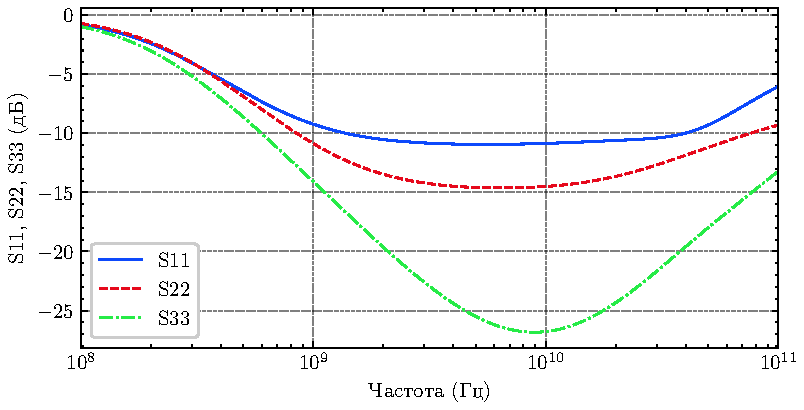
\includegraphics[width=0.8\linewidth]{lna_s11_s22.pdf}
	
	\caption{Результаты моделирования возвратных потерь по входу и выходу рассматриваемого МШУ}
	\label{ct:lna_s11_s22}
\end{figure}

\begin{figure}[ht]
	\centering
	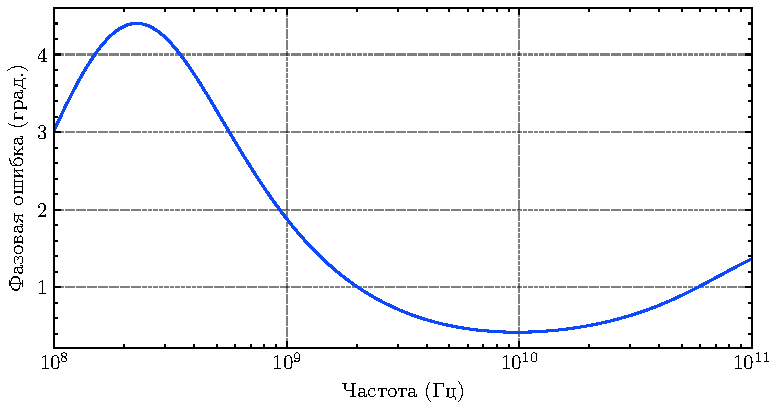
\includegraphics[width=0.8\linewidth]{phase_diff.pdf}
	
	\caption{Разница фаз между диффиренциальными компонентами на выходе рассматриваемого МШУ согласно результатам моделирования}
	\label{ct:phase_diff}
\end{figure}

\begin{figure}[ht]
	\centering
	\begin{circuitikz}[american, scale=1, transform shape]
		\def\killdepth#1{{\raisebox{0pt}[\height][0pt]{#1}}} \path (0,0) -- (2,0); % bounding box
		\ctikzset{transistors/arrow pos=end}
		\ctikzset{transistors/scale=1}
		
		\draw (0,0) node[left]{\(v_{RF+}\)} [short, o-] to [C, capacitors/scale=0.8] ++(2,0) node[npn, anchor=B](Q1){Q1} coordinate(tmp);
		\draw (Q1.C) [short, -] to ++(0, 4) node[vcc](VCC){\(V_{CC} = 2.5~V\)};
		\draw (Q1.E) [short, -] to [R] ++(0,-2) node[npn, anchor=C](Q2){Q2} (Q2.E) node[ground](GND){} (Q2.B) [short, -] to (Q2.B |- Q2.C) to (Q2.C) node[circ]{};
		\draw (Q1.E) [short, *-] to ++(2,0) node[npn, anchor=B](Q3){Q3};
		\draw (Q3.E) [short, -] to ++(0,-1) to [R] ++(0,-2) node[ground](GND){};
		\draw (Q3.C) [short, -] to ++(0,1) node[circ]{} to ++(-1,0) node[npn, anchor=E](Q4){Q4} to ++(2,0) node[npn, anchor=E, xscale=-1](Q5){\scalebox{-1}[1]{Q5}};
		\draw (Q4.C) [short, -] to ++(0,1) to [R] ++(0,2) node[vcc](VCC){\(V_{CC}\)};
		\draw (Q5.B) node[npn, anchor=B](Q6){Q6};
		\draw (Q6.E) [short, -] to ++(1,0) node[circ]{} coordinate(tmp) to ++(0,-1) node[npn,anchor=C, xscale=-1](Q7){\scalebox{-1}[1]{Q7}};
		\draw (tmp) [short, -] to ++(1, 0) node[npn, anchor=E, xscale=-1](Q8){\scalebox{-1}[1]{Q8}};
		\draw (Q7.E) [short, -] to ++(0,-1) to [R] ++(0,-2) node[ground](GND){};
		\draw (Q3.E) node[circ]{} [short, -] to [R] (Q7.E) node[circ]{};
		\draw (Q3.E) ++(0,-1) coordinate(tmp) node[circ]{} [short, -] to [C] (tmp -| Q7.E) node[circ]{};
		\draw (Q8.C) [short, -] to ++(0,1) to [R] ++(0,2) node[vcc](VCC){\(V_{CC}\)} coordinate(VCC);
		
		\draw (Q5.C) [short, -] to ++(1.2,1.2) coordinate(tmp) to (tmp -| Q8.C) node[circ]{};
		\draw (Q6.C) [short, -] to ++(-1.2, 1.2) coordinate(tmp) to (tmp -| Q4.C) node[circ]{};
		
		\draw (Q5.B) node[circ]{} [short, -] to ++(0,-1) node[ocirc]{} ++(0, -0.3) node(a){\(v_{LO+}\)};
		\draw (Q4.B) [short, -] to ++(0, -1) node[ocirc]{} ++(0, -0.3) node(a){\(v_{LO-}\)};
		\draw (Q8.B) [short, -] to ++(0, -1) node[ocirc]{} ++(0, -0.3) node(a){\(v_{LO-}\)};
		
		\draw (Q7.B) [short, -] to ++(2, 0) node[circ]{} node[npn, anchor=E, xscale=-1](Q9){\scalebox{-1}[1]{Q9}};
		\draw (Q9.E) [short, -] to [R] ++(0,-2) node[npn, anchor=C, xscale=-1](Q10){\scalebox{-1}[1]{Q10}} (Q10.E) node[ground]{} (Q10.B) [short, -] to (Q10.B |- Q10.C) to (Q10.C) node[circ]{};
		\draw (Q9.C) [short, -] to ++(0, 4) node[vcc]{\(V_{CC}\)};
		\draw (Q9.B) [short, -o] to [C, capacitors/scale=0.8] ++(2,0) node[right]{\(v_{RF-}\)};
		
		%COOOOOORDS
		\path (tmp) \coord(tmp);
	\end{circuitikz}
	
	\caption{Схема электрическая принципиальная сверхширокополосного смесителя}
	\label{ct:mixer_1_18}
\end{figure}

\begin{figure}[ht]
	\centering
	\begin{circuitikz}[american, scale=1, transform shape]
		\def\killdepth#1{{\raisebox{0pt}[\height][0pt]{#1}}} \path (0,0) -- (2,0); % bounding box
		
		\ctikzset{bipoles/amp/width=1.2}
		\draw (0,0) to[amp,t=LNA,l_=$F{=}12\,$dB, o-] ++(4,0);
		
		%COOOOOORDS
		%\path (tmp) \coord(tmp);
	\end{circuitikz}
	
	\caption{Структурная схема тракта приемника МИЧ \numrange{1}{1.8} ГГц и \numrange{1.8}{3.3} ГГц}
	\label{ct:struct_1_8_3_3}
\end{figure}

\begin{figure}[ht]
	\centering
	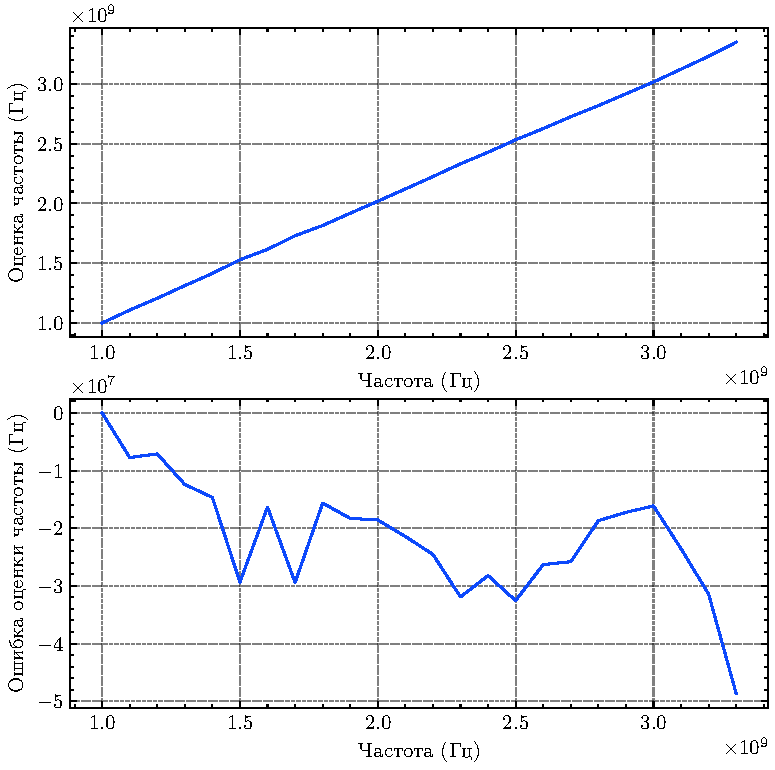
\includegraphics[width=0.7\linewidth]{fig.pdf}
	
	\caption{Оценка частоты тракта \numrange{1}{1.8} ГГц и \numrange{1.8}{3.3} ГГц}
	\label{ct:freq_estimate_1g_3g3}
\end{figure}

\begin{figure}[ht]
	\centering
	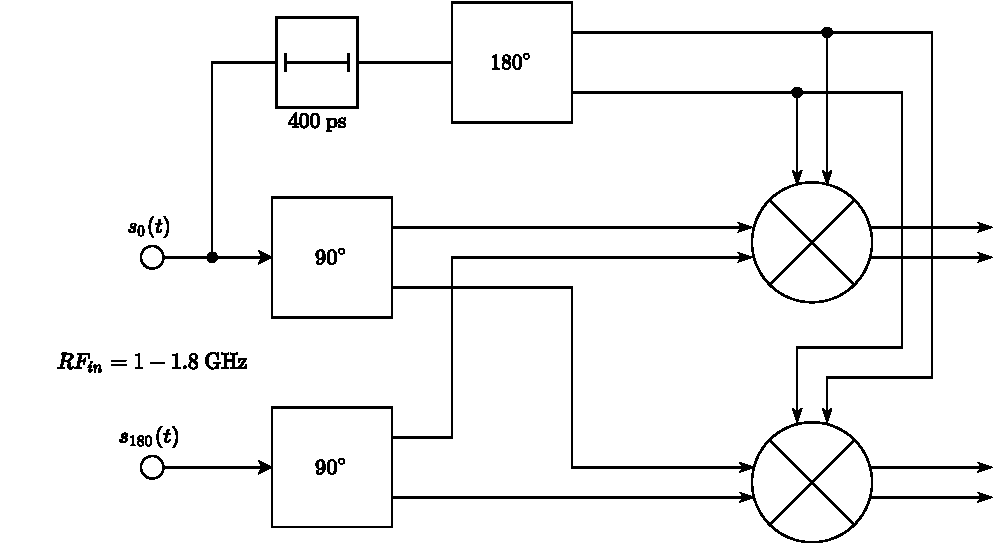
\includegraphics[width=0.6\linewidth]{IFM_Struct.pdf}
	
	\caption{Структурная схема частотного дискриминатора диапазона \numrange{1}{1.8} ГГц и \numrange{1.8}{3.3}}
	\label{ct:freq_estimate_1g_1g8}
\end{figure}

\begin{figure}[ht]
	\centering
	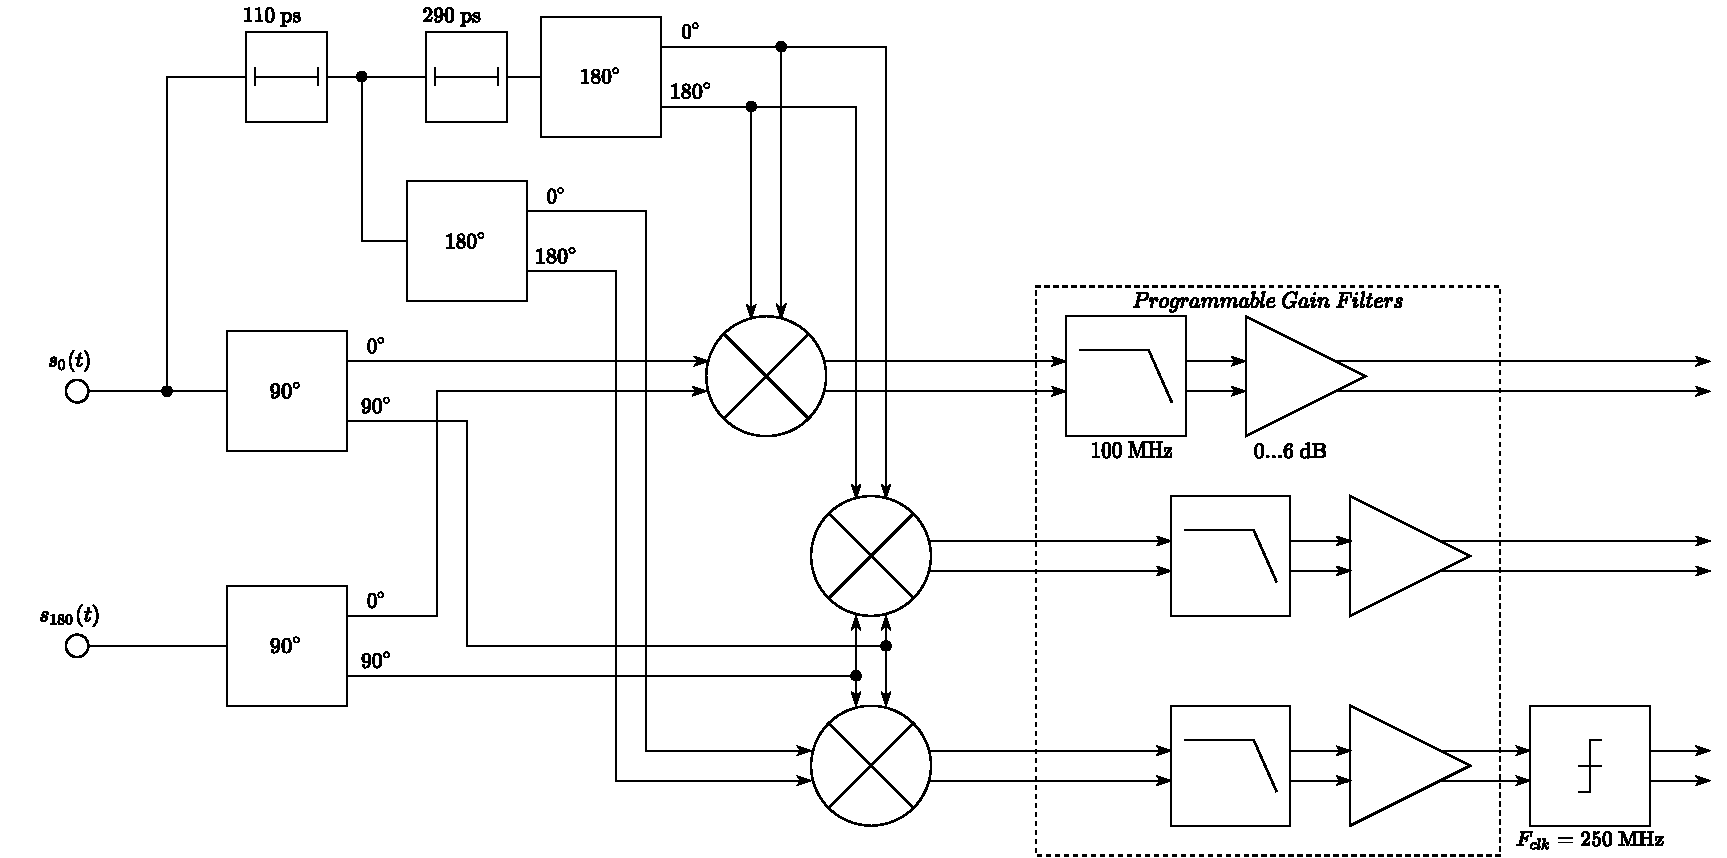
\includegraphics[width=1\linewidth]{IFM_Struct2.pdf}
	
	\caption{Структурная схема частотного дискриминатора диапазона \numrange{3.3}{6.3} ГГц}
	\label{ct:freq_estimate_3g3_6g3}
\end{figure}

\begin{figure}[ht]
	\centering
	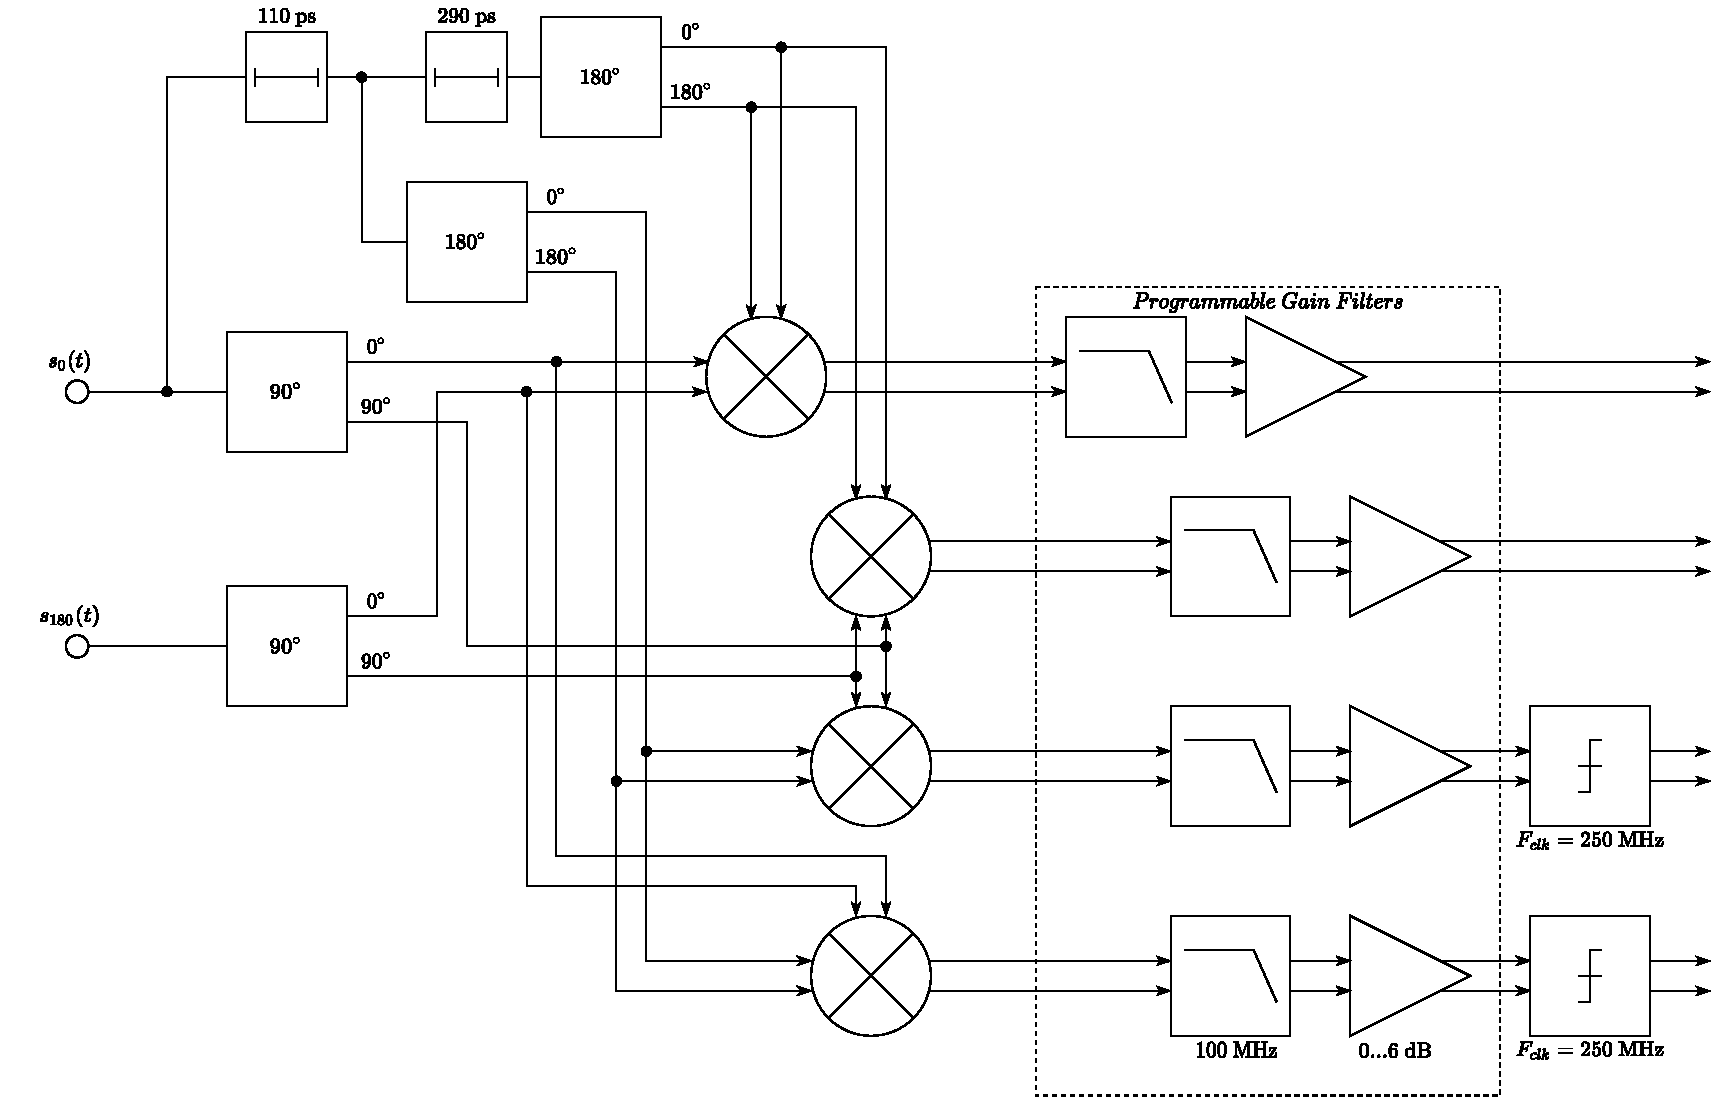
\includegraphics[width=1\linewidth]{IFM_Struct3.pdf}
	
	\caption{Структурная схема частотного дискриминатора диапазона \numrange{6.3}{12} ГГц}
	\label{ct:freq_estimate_6g3_12g}
\end{figure}